\chapter{Dataset}
Ai fini della tesi, il primo passo necessario per poter valutare correttamente la sinergia Apprendimento Continuo -- Human State Monitoring è ottenere raccolte di dati riguardanti quest'ultimo. I dati dovrebbero provenire da più soggetti, per correttezza statistica, e riguardare diversi aspetti biometrici della persona: battito cardiaco, sudorazione, respirazione, ecc.\\\\
I dataset selezionati ai fini di questa comparazione sono due, presentati nel dettaglio di seguito. In particolare, nella sezione 2.1 viene introdotto il dataset WESAD e il preprocessing eseguito nella sezione 2.1.1, mentre nella sezione 2.2 introduciamo il dataset ASCERTAIN, con il preprocessing dettagliato all'interno della sezione 2.2.1. Infine, nella sezione 2.3, vengono presentate le principali differenze fra i due dataset precedentemente descritti.
\section{WESAD}
Il dataset WESAD$^{\cite{10.1145/3242969.3242985}}$, acronimo di \textit{WEarable Stress and Affect Detection}, contiene dati raccolti da 15 soggetti durante uno studio effettuato in laboratorio riguardante i livelli di stress misurati tramite sensori biometrici e di movimento indossabili. Il dataset classifica questi dati in tre scale: neutralità, stress e divertimento.\\
I dispositivi usati per la raccolta dei dati sono due: uno indossato sul petto (RespiBAN) e uno indossato sul polso (Empatica E4).\\\\
\pagebreak

Il RespiBAN, indossato sul petto, raccoglie dati campionati a 700 Hz su:
\begin{itemize}
    \item[-] Elettrocardiogramma (ECG)
    \item[-] Attività elettrodermica (EDA)
    \item[-] Elettromiogramma (EMG)
    \item[-] Respirazione
    \item[-] Temperatura corporea
    \item[-] Accelerazione sui tre assi
\end{itemize}
L'Empatica E4, indossato sul polso, monitora con frequenza di campionamento eterogenea:
\begin{itemize}
    \item[-] Pulsazioni (BVP), a 64Hz
    \item[-] Attività elettrodermica (EDA), a 4 Hz
    \item[-] Temperatura corporea, a 4 Hz
    \item[-] Accelerazione sui tre assi, a 32 Hz
\end{itemize}
La quantità di dati contenuti in questo dataset lo rende un ottimo strumento nell'addestramento di modelli di Machine Learning riguardanti l'ambiente dello HSM. Dati come le pulsazioni, la temperatura e l'elettrocardiogramma sono precisissimi indicatori biometrici dello stato psico-fisico di una persona e pertanto sono estremamente utili alle reti neurali per dedurre lo stato psico-fisico di soggetto.
\subsection{Preprocessing}
Una volta caricato il dataset, i dati sono stati concatenati e ricampionati a 32 Hz, attraverso la libreria \texttt{SciPy}.
\lstinputlisting[style=myPython, firstnumber=31, firstline=31, lastline=42]{code/wesad_data.py}
Dopodiché, l'insieme delle features è stato standardizzato ponendo media pari a 0 e deviazione standard uguale a 1
\lstinputlisting[style=myPython, firstnumber=46, firstline=46, lastline=46]{code/wesad_data.py}
Sono state ricampionate le etichette e sono state rimosse l'etichetta 0, corrispondente ad una condizione di neutralità, e le etichette 5, 6 e 7 poichè secondo le indicazioni del dataset sono corrispondenti a dati da ignorare.
\lstinputlisting[style=myPython, firstnumber=50, firstline=50, lastline=52]{code/wesad_data.py}
\lstinputlisting[style=myPython, firstnumber=56, firstline=56, lastline=57]{code/wesad_data.py}
\lstinputlisting[style=myPython, firstnumber=86, firstline=86, lastline=87]{code/wesad_data.py}
I dati sono poi raccolti in sottosequenze di 100 punti relativi alla stessa etichetta, corrispondenti a circa 3 secondi, e per ogni etichetta vengono estratte 100 di queste sottosequenze.
\lstinputlisting[style=myPython, firstnumber=62, firstline=62, lastline=82]{code/wesad_data.py}
Dai dati viene poi estratto un test set. Questo ci lascia con un test set di 1500 elementi e un training set da 4500 elementi suddivisi come specificato nella tabella \ref{tab:splittedwesad}.

\section{ASCERTAIN}
ASCERTAIN$^{\cite{10.1145/2818346.2820736}}$, acronimo di \textit{multimodal databASe for impliCit pERsonaliTy and Affect recognitIoN}, è un dataset contenente dati provenienti da 58 soggetti raccolti con sensori fisiologici commerciali e classifica le informazioni su diverse scale: incitamento, valenza, investimento, apprezzamento e familiarità. Il dataset contiene anche dati relativi all'attività facciale dei soggetti registrati con sensori comuni, oltre ai dati sull'elettroencefalogramma (EEG), elettrocardiogramma (ECG) e sulle risposte galvaniche della pelle (GSR).\\\\
ASCERTAIN è un dataset contenente molti più dati rispetto a WESAD, raccolti con dispositivi commerciali comuni, il che rende questa raccolta di dati molto utile per poter valutare l'applicazione di metodologie di Apprendimento Continuo. Usando dispositivi commerciali si può simulare un contesto più vicino all'ambiente di produzione che ad un esperimento controllato in laboratorio.
\subsection{Preprocessing}
Dal dataset sono stati esclusi due soggetti poiché i loro dati risultavano imprecisi o incompleti. Ogni soggetto rimanente è stato caricato e per ognuno sono state create le etichette seguendo la seguente suddivisione basata sui valori di incitamento e valenza specificati, che corrispondono ai quadranti del grafico cartesiano creato dai due valori:
\begin{itemize}
    \item[-] Label 0, corrispondente a valori di incitamento $> 3$ e valenza $> 0$
    \item[-] Label 1, corrispondente a valori di incitamento $> 3$ e valenza $\leq 0$
    \item[-] Label 2, corrispondente a valori di incitamento $\leq 3$ e valenza $> 0$
    \item[-] Label 3, corrispondente a valori di incitamento $\leq 3$ e valenza $\leq 0$
\end{itemize}
\lstinputlisting[style=myPython, firstnumber=40, firstline=40, lastline=51]{code/ascertain_data2.py}
I dati sono poi ripuliti dai valori mancanti, ricampionati a 32 Hz e concatenati fra loro.
\lstinputlisting[style=myPython, firstnumber=55, firstline=55, lastline=58]{code/ascertain_data2.py}
\lstinputlisting[style=myPython, firstnumber=62, firstline=62, lastline=64]{code/ascertain_data2.py}
\lstinputlisting[style=myPython, firstnumber=68, firstline=68, lastline=76]{code/ascertain_data2.py}
Vengono poi costruite le sottosequenze, da 160 elementi ciascuna (5 secondi), mantenendo un bilanciamento fra le diverse classi.
\lstinputlisting[style=myPython, firstnumber=80, firstline=80, lastline=80]{code/ascertain_data2.py}
\lstinputlisting[style=myPython, firstnumber=82, firstline=82, lastline=104]{code/ascertain_data2.py}
Analogamente a WESAD, anche da ASCERTAIN viene estratto un test set. A preprocessing ultimato, il dataset è suddiviso in un test set da 720 elementi e un training set da 2160 elementi suddivisi come indicato nella Tabella \ref{tab:splittedascertain}

\begin{table}[h]
\small
    \parbox{.45\linewidth}{
    	\begin{center}
    		\begin{tabular}{l|c}
    		     \textbf{Soggetto} & \textbf{Dati}\\
    		     \hline
    		     S2 & 287 \\
    		     S3 & 287 \\
    		     S4 & 298 \\
    		     S5 & 298 \\
    		     S6 & 297 \\
    		     S7 & 303 \\
    		     S8 & 309 \\
    		     S9 & 292 \\
    		     S10 & 313 \\
    		     S11 & 292 \\
    		     S13 & 308 \\
    		     S14 & 297 \\
    		     S15 & 305 \\
    		     S16 & 313 \\
    		     S17 & 301 \\
    		     \hline
    		     Totale & 4500\\
    		     \multicolumn{1}{c}{}\\
    		     \multicolumn{1}{c}{}
    		\end{tabular}
    		\caption{Datataset WESAD}
    		\label{tab:splittedwesad}
    	\end{center}
	}
    \parbox{.45\linewidth}{
    	\begin{center}
    		\begin{tabular}{l|c}
    		     \textbf{Soggetto} & \textbf{Dati}\\
    		     \hline
    		     S0 & 95 \\
    		     S1 & 75 \\
    		     S2 & 148 \\
    		     S3 & 154 \\
    		     S4 & 153 \\
    		     S5 & 208 \\
    		     S6 & 131 \\
    		     S7 & 115 \\
    		     S8 & 119 \\
    		     S9 & 206 \\
    		     S10 & 119 \\
    		     S11 & 78 \\
    		     S12 & 74 \\
    		     S13 & 109 \\
    		     S14 & 72 \\
    		     S15 & 84 \\
    		     S16 & 220 \\
    		     \hline
    		     Totale & 2160
    		\end{tabular}
    		\caption{Datataset ASCERTAIN}
    		\label{tab:splittedascertain}
    	\end{center}
    }
\end{table}
\section{Differenze fra i due dataset}
Uno degli elementi da considerare quando si addestra una rete neurale è il bilanciamento dei dati presi in considerazione per l'addestramento.\\
Andando ad analizzare nel dettaglio la struttura dei due dataset considerati, diventa evidente la decisa sovrarappresentanza della classe 0 nel dataset ASCERTAIN (Figura \ref{fig:ascertainclasses}), mentre le classi nel dataset WESAD risultano molto più bilanciate (Figura \ref{fig:wesadclasses}). Questo è anche dovuto all'aver scelto delle classi fittizie, per quanto riguarda ASCERTAIN, che ha evidenziato come non tutti i soggetti abbiano prodotto dati bilanciati rispetto alle nuove classi selezionate. Anche eseguendo un bilanciamento successivo, ovvero eliminando gli esempi in eccesso sulla prima classe, si raggiungono misurazioni analoghe a quelle presentate.\\\\
Bilanciando il dataset ASCERTAIN attraverso la produzione di soggetti fittizi, ognuno contenente dati presi da tutti i soggetti in maniera bilanciata rispetto alle nuove classi, otteniamo immediatamente risultati sensibilmente migliori, con accuratezze a volte anche doppie rispetto allo stesso metodologia sul dataset ASCERTAIN originale. Questo rende evidente l'importanza dell'avere dati di addestramento bilanciati, quindi esempi in quantità simile per ognuna delle etichette possibili.
\begin{figure}[h]
    \begin{minipage}[b]{0.5\textwidth}
		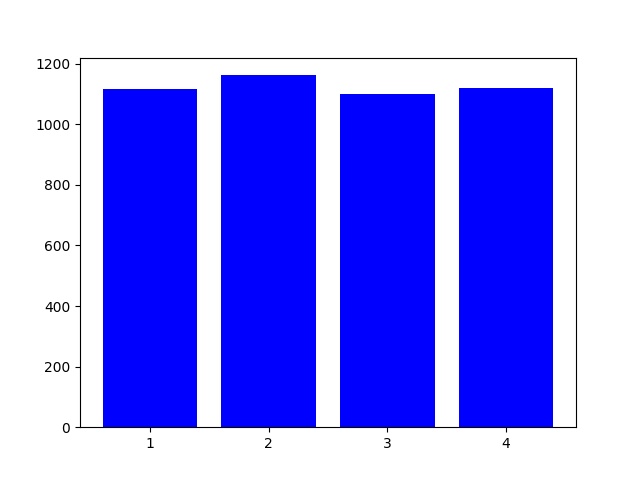
\includegraphics[width=\textwidth]{img/graphs/wesad_dataset.png}
		\caption{Presenza delle classi su dataset WESAD}
		\label{fig:wesadclasses}
	\end{minipage}
    \hfill
    \begin{minipage}[b]{0.5\textwidth}
		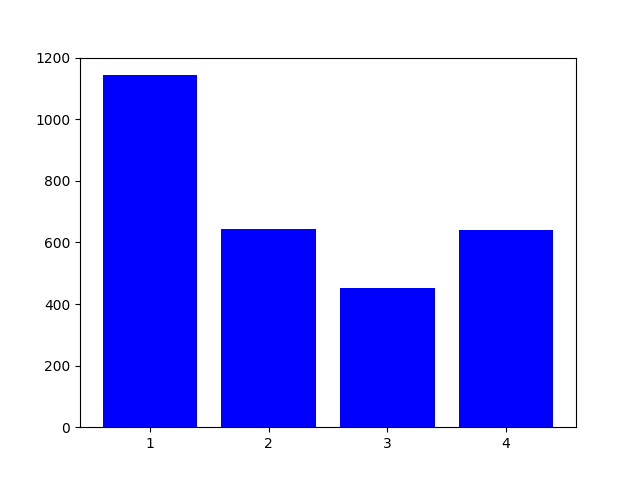
\includegraphics[width=\textwidth]{img/graphs/ascertain_dataset.png}
		\caption{Presenza delle classi su dataset ASCERTAIN}
		\label{fig:ascertainclasses}
	\end{minipage}
\end{figure}